\section[Naive Bayes Algorithm]{Naive Bayes Algorithm}

\subsection[Use Case]{Use Case}

\begin{frame}{Presentation of the Use Case}
	We will use text data as our support: movie reviews, in order to perform \textbf{sentiment analysis}.
	\begin{itemize}
		\item We will use a database of movie reviews posted by users on the English-speaking website \href{https://m.imdb.com/}{IMDb}: \url{https://www.kaggle.com/datasets/yasserh/imdb-movie-ratings-sentiment-analysis}
		\item These reviews are either positive or negative.
		\item We will therefore build a binary classifier to map a review to an opinion (positive or negative).
	\end{itemize}
	A Naive Bayes algorithm is an excellent candidate for this type of problem! 
\end{frame}

\begin{frame}{Challenge}
	There is a double challenge!
	\begin{itemize}
		\item How do we process text data using a machine learning algorithm?
		\item How can we apply Bayes' theorem to this data?
	\end{itemize}
\end{frame}

\begin{frame}{Working Data}
	Suppose we have collected examples of positive and negative reviews. We have \textbf{counted} how many times certain words appear in the reviews:
	\begin{columns}
		\begin{column}{0.5\textwidth}
			\begin{figure}
				\centering
				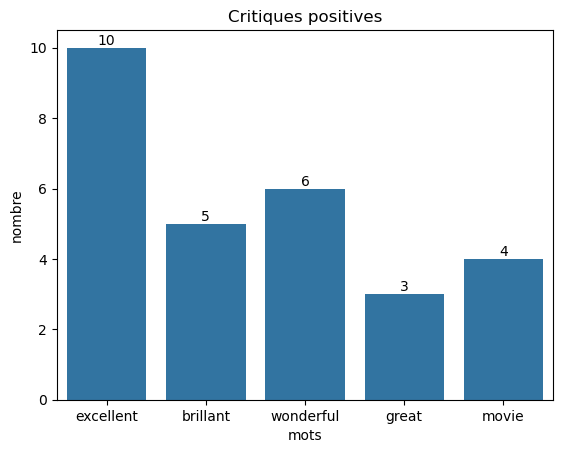
\includegraphics[width=1.0\linewidth]{Images/critiques_positives}
				\label{fig:critiques_positives}
			\end{figure}
		\end{column}
		\begin{column}{0.5\textwidth}
			\begin{figure}
				\centering
				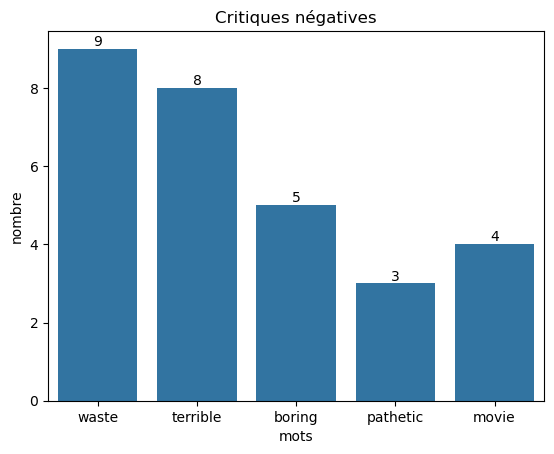
\includegraphics[width=1.0\linewidth]{Images/critiques_negatives}
				\label{fig:critiques_negatives}
			\end{figure}
		\end{column}		
	\end{columns}	
\end{frame}

\begin{frame}{Working Data - Probabilities}
	We can easily derive \textbf{conditional probabilities} from this data. They are conditional in the sense that we process positive reviews and negative reviews separately:
	\begin{columns}
		\begin{column}{0.5\textwidth}
			\begin{figure}
				\centering
				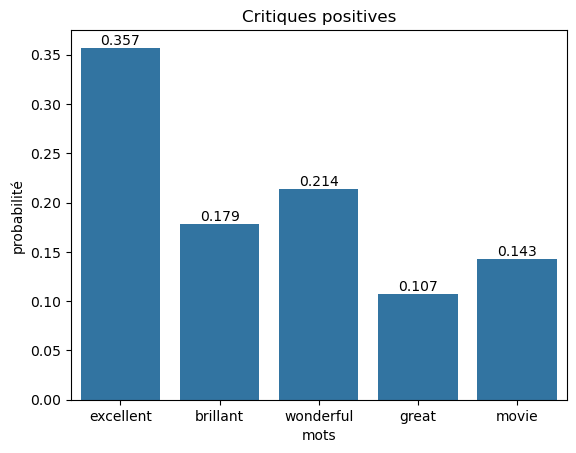
\includegraphics[width=1.0\linewidth]{Images/critiques_positives_probab}
				\label{fig:critiques_positives_probab}
			\end{figure}
		\end{column}
		\begin{column}{0.5\textwidth}
			\begin{figure}
				\centering
				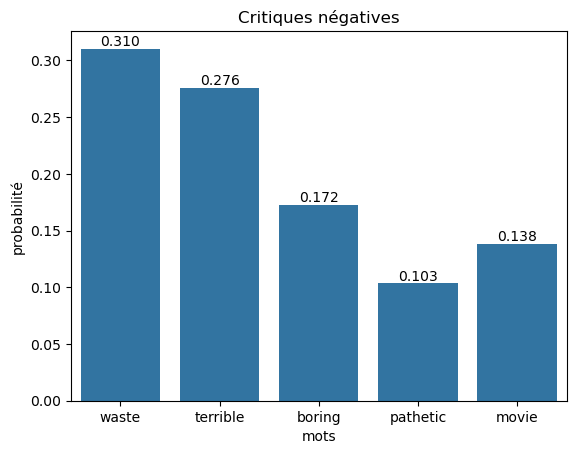
\includegraphics[width=1.0\linewidth]{Images/critiques_negatives_probab}
				\label{fig:critiques_negatives_probab}
			\end{figure}
		\end{column}		
	\end{columns}	
\end{frame}

\begin{frame}{First Calculation Attempt}
	\begin{itemize}
		\item We will denote by $C$ the discrete random variable $C \in \{0, 1\}$ that represents the sentiment associated with a review.
		\item $C$ equals 1 if the review is positive and 0 otherwise. Suppose the prior probability is balanced: $P(C = 0) = 0.5$ and $P(C = 1) = 0.5$.
		\item The review we are interested in is the following: \textit{brilliant}. How do we compute a posterior probability?
	\end{itemize}
	\pause
	One way to proceed would be to calculate the Bayes factor:
	\begin{equation}
		\text{BF}_{10}(\text{"brilliant"}) = \frac{P(\text{"brilliant"} \mid C = 1)}{P(\text{"brilliant"} \mid C = 0)}
		\nonumber
	\end{equation}
	But there is a minor problem: $P(\text{"brilliant"} \mid C = 0) = 0$. This would lead to an infinite Bayes factor!
\end{frame}

\begin{frame}{Working Data - Laplace Smoothing}
	We will transform the data using \textbf{Laplace smoothing}. Instead of computing the conditional probabilities like this:
	\begin{equation}
		P(\text{word} \mid C = K) = \frac{\text{number of occurrences of word when } C = K}{\text{total number of occurrences when }C = K}
		\nonumber
	\end{equation}
	\pause
	We will compute them like this:
	\begin{equation}
		\begin{split}
			&P(\text{word} \mid C = K) = \\
			&\frac{\text{number of occurrences of word when } C = K + \color{red}1}{\text{total occurrences when } C = K + \color{red} \text{total number of unique words}}
		\end{split}
		\nonumber
	\end{equation}
	\pause
	This simply consists of adding each word once to the set of classes (positive review and negative review).
\end{frame}

\begin{frame}{Working Data - Laplace Smoothing}
	Once Laplace smoothing is applied, we obtain:
	\begin{columns}
		\begin{column}{0.5\textwidth}
			\begin{figure}
				\centering
				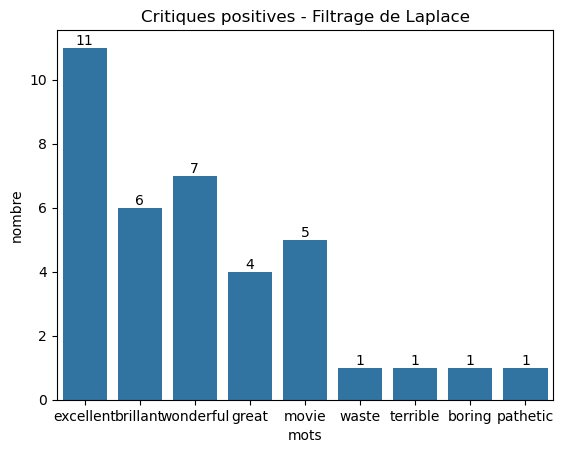
\includegraphics[width=1.0\linewidth]{Images/critiques_positives_laplace}
				\label{fig:critiques_positives_laplace}
			\end{figure}
		\end{column}
		\begin{column}{0.5\textwidth}
			\begin{figure}
				\centering
				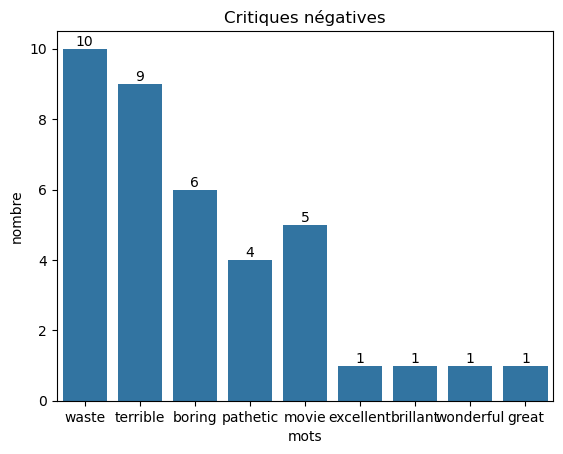
\includegraphics[width=1.0\linewidth]{Images/critiques_negatives_laplace}
				\label{fig:critiques_negatives_laplace}
			\end{figure}
		\end{column}		
	\end{columns}	
\end{frame}

\begin{frame}{Working Data - Probabilities with Laplace Smoothing}
	And the updated conditional probabilities:
	\begin{columns}
		\begin{column}{0.5\textwidth}
			\begin{figure}
				\centering
				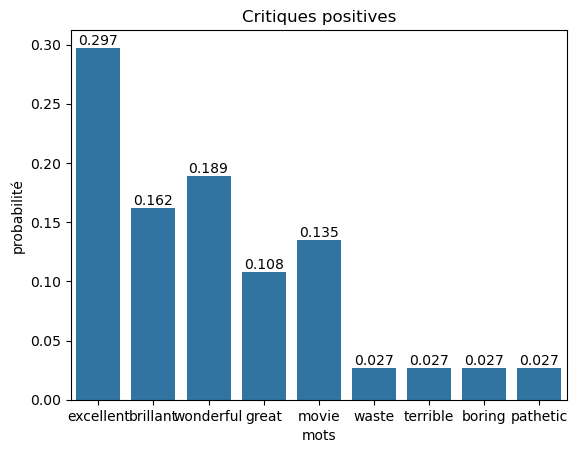
\includegraphics[width=1.0\linewidth]{Images/critiques_positives_probab_laplace}
				\label{fig:critiques_positives_probab_laplace}
			\end{figure}
		\end{column}
		\begin{column}{0.5\textwidth}
			\begin{figure}
				\centering
				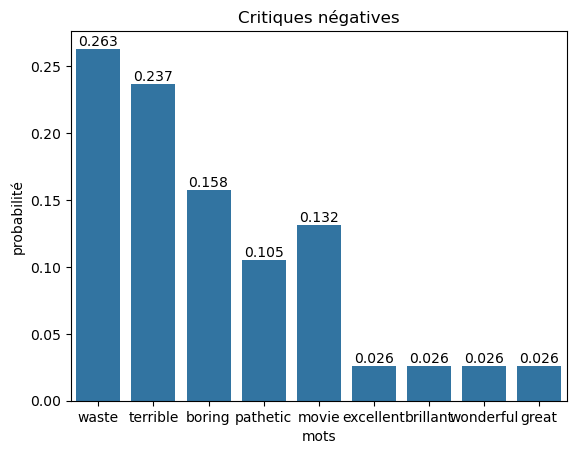
\includegraphics[width=1.0\linewidth]{Images/critiques_negatives_probab_laplace}
				\label{fig:critiques_negatives_probab_laplace}
			\end{figure}
		\end{column}		
	\end{columns}	
\end{frame}

\subsection[Probability Calculations]{Probability Calculations}

\begin{frame}{First Calculation}
	\begin{itemize}
		\item Suppose the prior probability is balanced: $P(C = 0) = 0.5$ and $P(C = 1) = 0.5$.
		\item The review we are interested in is the following: \textit{brilliant}. How do we compute a posterior probability?
	\end{itemize}
	\pause
	One way to proceed would be to calculate the Bayes factor:
	\begin{equation}
		\begin{aligned}
			\text{BF}_{10}(\text{"brilliant"}) 
			&= \frac{P(\text{"brilliant"} \mid C = 1)}{P(\text{"brilliant"} \mid C = 0)} \\
			&= \frac{0.162}{0.026} \approx 6.23
		\end{aligned}
		\nonumber
	\end{equation}
	\pause
	Since the initial odds are $1:1$, the final odds become $6.23:1$. This results in a posterior probability of 0.862.
\end{frame}

\begin{frame}{First Calculation - Alternative}
	An alternative consists of computing the following 2 quantities, which correspond to the numerators in Bayes' theorem:
	\begin{equation}
		\begin{cases}
			P(\text{"brilliant"} \mid C = 1) P(C=1) \\
			P(\text{"brilliant"} \mid C = 0) P(C=0)
		\end{cases}
		\nonumber
	\end{equation}
	\pause
	We do not need to worry about the denominator $P(\text{"brilliant"})$, given that the sum of the posterior probabilities must equal 1:
	\begin{equation}
		\begin{cases}
			P(C = 1 \mid \text{"brilliant"}) \propto P(\text{"brilliant"} \mid C = 1) P(C=1) \\
			P(C = 0 \mid \text{"brilliant"}) \propto P(\text{"brilliant"} \mid C = 0) P(C=0)
		\end{cases}
		\nonumber
	\end{equation}
	This is the approach implemented in the Naive Bayes algorithm.
\end{frame}

\begin{frame}{First Calculation - Alternative}
	We can verify that this leads to the same result:
	\begin{equation}
		\begin{cases}
			P(\text{"brilliant"} \mid C = 1) P(C=1) = 0.162 \times 0.5 = 0.081 \\
			P(\text{"brilliant"} \mid C = 0) P(C=0) = 0.026 \times 0.5 = 0.013
		\end{cases}
		\nonumber
	\end{equation}	
	After normalization, we obtain:
	\begin{equation}
		\begin{cases}
			P(C = 1 \mid \text{"brilliant"}) = 0.081 / (0.081 + 0.013) =  0.862 \\
			P(C = 0 \mid \text{"brilliant"}) = 0.013 / (0.081 + 0.013) =  0.138
		\end{cases}
		\nonumber
	\end{equation}
	We obtain, naturally, the exact same result. This is the standard method implemented in a Naive Bayes algorithm.
\end{frame}

\subsection[Naive Bayes Algorithm Assumptions]{Naive Bayes Algorithm Assumptions}

\begin{frame}{A More Elaborate Review}
	Suppose now that the review is \textit{boring movie, waste of time}:
	\begin{itemize}
		\item The words \textit{of} and \textit{time} are not part of the \textbf{vocabulary} we considered.
		\pause
		\item We will therefore ignore these terms.
		\pause
		\item Punctuation is also not handled, so we will remove it. The review thus becomes \textit{boring movie waste}.
		\pause
		\item We seek to compute: $P(C = 1 \mid \text{"boring movie waste"})$, which requires knowing the likelihood $P(\text{"boring movie waste"} \mid C = 1)$.
		\pause
		\item However, we do not know the joint probability of these words! They are inherently dependent. A sentence is not just a random stack of words.
	\end{itemize}
	\pause
	This is where the \textbf{naive} nature of the algorithm comes into play. To simplify, we assume that words within the same sentence are independent. This is \textbf{false}, but it drastically simplifies the calculations!
\end{frame}

\begin{frame}{Naive Nature of the Algorithm}
	\begin{itemize}
		\item This is where the \textbf{naive} nature of the algorithm plays its part.
		\pause
		\item To simplify, we will assume that words within the same sentence are independent.
		\pause
		\item This is \textbf{simplistic}, but highly practical for performing calculations!
	\end{itemize}
	\pause
	\vspace{0.5cm}
	This mirrors all the examples covered so far. We assumed that Covid-19 tests were independent, as well as the movie reviews. And here, we treat the words within the same sentence as independent!
\end{frame}

\begin{frame}{Multinomial Nature of the Algorithm}
	\begin{itemize}
		\item Recall that our simplified review is: \textit{boring movie waste}.
		\pause
		\item We treat each word as independent. Therefore, it requires performing 3 updates with Bayes' theorem, or multiplying 3 Bayes factors.
		\pause
		\item The difference from our previous examples is that each word brings a \textbf{different} weight of evidence: the Bayes factors are unique for each word, which is the novelty.
		\pause
		\item For this reason, this algorithm is called the \textbf{multinomial} Naive Bayes algorithm. 
		\pause
		\item "Multinomial" refers to the nature of the probability distribution. Our previous examples used a Bernoulli distribution!
		\pause
		\item Our algorithm utilizes 2 multinomial distributions: one for negative reviews and one for positive reviews. The probability plots seen earlier are actually the probability mass functions (PMFs) of these distributions!
	\end{itemize}
\end{frame}

\begin{frame}{A More Elaborate Review - Calculation}
	\begin{equation}
		\resizebox{1.0\textwidth}{!}{%
			$\begin{cases}
				P(C = 0 \mid \text{"boring movie waste"}) \propto P(\text{"boring movie waste"} \mid C = 0) P(C=0) \\
				P(C = 1 \mid \text{"boring movie waste"}) \propto P(\text{"boring movie waste"} \mid C = 1) P(C=1)
			\end{cases}$
		}
		\text{\quad or \quad}
		\resizebox{1.0\textwidth}{!}{%
			$\begin{cases}
				P(C = 0 \mid \text{"boring movie waste"}) \propto P(\text{"boring movie waste"} \mid C = 0) P(C=0) \\
				P(C = 1 \mid \text{"boring movie waste"}) \propto P(\text{"boring movie waste"} \mid C = 1) P(C=1)
			\end{cases}$
		}
		\nonumber
	\end{equation}
	\pause
	With the naive independence assumption, we can write:
	\begin{equation}
		\begin{aligned}
			&P(\text{"boring movie waste"} \mid C = 0) P(C=0) \\
			&= P(\text{"boring"} \mid C = 0) P(\text{"movie"} \mid C = 0) P(\text{"waste"} \mid C = 0) P(C=0) \\
			&= 0.158 \times 0.132 \times 0.263 \times 0.5 \\
			&\approx 0.00274 
		\end{aligned}
		\nonumber
	\end{equation}
	\pause
	Similarly:
	\begin{equation}
		\begin{aligned}
			&P(\text{"boring movie waste"} \mid C = 1) P(C=1) \\
			&= P(\text{"boring"} \mid C = 1) P(\text{"movie"} \mid C = 1) P(\text{"waste"} \mid C = 1) P(C=1) \\
			&= 0.027 \times 0.135 \times 0.027 \times 0.5 \\
			&\approx 0.00005
		\end{aligned}
		\nonumber
	\end{equation}
\end{frame}

\begin{frame}{A More Elaborate Review - Calculation}
	After normalization, we obtain:
	\begin{equation}
		\begin{cases}
			P(C = 0 \mid \text{"boring movie waste"}) \approx 0.982 \\
			P(C = 1 \mid \text{"boring movie waste"}) \approx 0.018
		\end{cases}
		\nonumber
	\end{equation}
	\pause
	Multiplying probabilities quickly leads to very small numbers. Algorithms therefore compute the \textbf{logarithms} of probabilities. Thanks to the independence assumption, the logarithm of a product of probabilities becomes the sum of the logarithms of the individual probabilities.
\end{frame}

\begin{frame}{A More Elaborate Review - Bayes Factors}
	We can calculate the Bayes factors for each word:
	\begin{equation}
		\begin{cases}
			\text{BF}_{10}(\text{"boring"}) = P(\text{"boring"} \mid C = 1) / P(\text{"boring"} \mid C = 0) \approx 0.171 \\
			\text{BF}_{10}(\text{"movie"}) = P(\text{"movie"} \mid C = 1) / P(\text{"movie"} \mid C = 0) \approx 1.023 \\
			\text{BF}_{10}(\text{"waste"}) = P(\text{"waste"} \mid C = 1) / P(\text{"waste"} \mid C = 0) \approx 0.103
		\end{cases}
		\nonumber
	\end{equation}
	\pause
	\begin{itemize}
		\item The word \textit{movie} will have very little influence on the final result because its Bayes factor is very close to 1.
		\item The word \textit{waste} provides the strongest evidence that the review is negative.
		\item We can easily derive the Bayes factors by dividing the two PMFs of the multinomial distributions.
	\end{itemize}
\end{frame}

\subsection[Formulation of the Naive Bayes Algorithm]{Formulation of the Naive Bayes Algorithm}

\begin{frame}{Conditional Independence Assumption}
	Let $x \in \R^d$ be an input feature vector and $C \in \{0, 1\}$ a discrete random variable.
	\vspace{0.3cm}
	\begin{block}{Conditional Independence Assumption (Naive)}
		We assume that the elements of $x$ are conditionally independent given the class:
		\begin{equation}
			P(x_1, x_2, \cdots, x_d \mid C = k) = \prod_{i=1}^{d} P(x_i \mid C = k) \quad k \in \{0, 1\}
			\nonumber
		\end{equation}
	\end{block}
\end{frame}

\begin{frame}{Maximum A Posteriori}
	\begin{block}{Decision Rule (Maximum A Posteriori)}
		We search for the class that maximizes the product of the prior probability and the likelihood:
		\begin{equation}
			\hat{y} = \argmax{k \in \{0, 1\}} \left( P(C = k) \prod_{i=1}^{d} P(x_i \mid C = k) \right)
			\nonumber
		\end{equation}
	\end{block}
	\pause
	Note: The naive assumption \textit{biases} the posterior probability estimates; however, since we only seek the maximum a posteriori class, the impact of this simplistic assumption remains limited in practical applications.
\end{frame}

\begin{frame}{Switching to Logarithms}
	To prevent numerical underflow errors and transform products into sums:
	\begin{block}{Decision Rule (Maximum A Posteriori)}
		We search for the class that maximizes the logarithm of the product of the prior probability and the likelihood:
		\begin{equation}
			\hat{y} = \argmax{k \in \{0, 1\}} \left( \log P(C = k) + \sum_{i=1}^{d} \log P(x_i \mid C = k) \right)
			\nonumber
		\end{equation}
	\end{block}
	\pause
	\begin{itemize}
		\item This matches the implementation found in \href{https://scikit-learn.org/stable/modules/generated/sklearn.naive_bayes.MultinomialNB.html}{\texttt{sklearn.naive\_bayes.MultinomialNB}}.
	\end{itemize}
\end{frame}

\begin{frame}{Probability Computation with the Softmax Function}
	Once the log-scores $\log P(C = k \mid x_1, \cdots, x_d)$ are computed, we can recover calibrated probabilities using a \textbf{softmax} function:
	\begin{equation}
		\resizebox{1.0\textwidth}{!}{%
			$P(C = 1 \mid x_1, \cdots, x_d) = \frac{\exp{\left(\log P(C = 1  \mid x_1, \cdots, x_d)\right)}}{\exp{\left(\log P(C = 1  \mid x_1, \cdots, x_d)\right)} + \exp{\left(\log P(C = 0  \mid x_1, \cdots, x_d)\right)}}$
		}
		\nonumber
	\end{equation}
\end{frame}

\subsection[Combining Algorithms]{Combining Algorithms}

\begin{frame}{Case Study}
	\begin{itemize}
		\item On the Université de Toulouse campus, we collect the height and the UFR (Academic Department) — such as the Faculty of Health, Humanities, Arts, or the Faculty of Science and Engineering — from a sample of students.
		\pause
		\item We have global statistics showing the gender baseline distribution: male students (40\%) and female students (60\%). This represents our prior probability.
		\pause
		\item We can establish two Gaussian distributions for the height of male and female students and use them within a Gaussian Naive Bayes framework.
		\pause
		\item We can establish two multinomial distributions for the UFR departments of male and female students and use them within a Multinomial Naive Bayes framework.
	\end{itemize}
\end{frame}

\begin{frame}{Case Study - Calculation}
	\begin{itemize}
		\item Suppose we look at a student whose height (172 cm) and UFR department (Humanities) are known. What is the probability that this student is female?
		\pause
		\item We can compute the likelihoods $\log P(\text{Humanities} \mid \text{Female})$ and $\log P(\text{Humanities} \mid \text{Male})$ using the multinomial distributions. In practice, this simply means reading the PMFs!
		\pause
		\item We can compute the likelihoods $\log P(\text{172 cm} \mid \text{Female})$ and $\log P(\text{172 cm} \mid \text{Male})$ using the Gaussian distributions.
		\pause
		\item We then add these log-likelihoods to their respective log-priors: $\log P(\text{Humanities} \mid \text{Female}) + \log P(\text{172 cm} \mid \text{Female}) + \log P(\text{Female})$
		\pause
		\item And similarly: $\log P(\text{Humanities} \mid \text{Male}) + \log P(\text{172 cm} \mid \text{Male}) + \log P(\text{Male})$. 
		\pause
		\item We pass these scores through the softmax function, and that's it!
	\end{itemize}
\end{frame}

\begin{frame}{Case Study - Details for the Gaussian Naive Bayes Algorithm}
	For a continuous variable (height), we no longer count occurrences. Instead, we use the \textbf{normal (Gaussian) distribution}:
	\begin{equation}
		P(x \mid C=k) = \frac{1}{\sqrt{2\pi\sigma_k^2}} \exp\left(-\frac{(x-\mu_k)^2}{2\sigma_k^2}\right)
		\nonumber
	\end{equation}
	\pause
	\begin{itemize}
		\item $\mu_k$: Mean height for class $k$ (e.g., 164 cm for female students, 176 cm for male students).
		\item $\sigma_k$: Standard deviation for class $k$.
	\end{itemize}
	\pause
	\vspace{0.3cm}
	The calculation in log space:
	\begin{equation}
		\log P(x \mid C=k) = -\frac{1}{2} \log(2\pi\sigma_k^2) - \frac{(x-\mu_k)^2}{2\sigma_k^2}
		\nonumber
	\end{equation}
	The closer the student's height is to the mean of a class, the higher this log-score will be.
\end{frame}